\chapter{Implementation og tests}
\section{Hej Mads}
\section{Hallo}

\subsection{Clock Manager}
In this entity the different clock signals are generated as dividers of the master on-board 50 MHz clock. \\ 
We generate two sub-clocks. One \texttt{clk} that runs at $50000000/(2^16) = 762.94$ Hz. And a slow clock \texttt{clk\_3} for the alarm-blink signal, which runs at $50000000/(2^24) = 2.98$ Hz.

\subsection{Input Synchronization and avoiding metastability}
All the inputs from the outside world must be synchronized to the clock. This is done to avoid meta-stability, which is a very undesirable condition in digital systems. Meta-stability can occur if an input value is changed too close to the clock edge violating either the setup- or holdtime of the gate. If the setup/hold times are violated, there is no way to tell if the input will go low or high, which of course is a problem in itself. The biggest problem however is not the uncertainty of whether the signal goes low or high, but the fact that there's no way of knowing exactly how long the value will be afloat between low and high. It is only possible to give probabilities of how long a metastable state will last. An example of metastability in practice can be seen on figure \ref{fig:meta}, where several experiments shows the uncertainty of the whether the signal is going high or low an more importantly the uncertainty of how long the metastable state lasts.\\

\begin{figure}[!h]
\centering
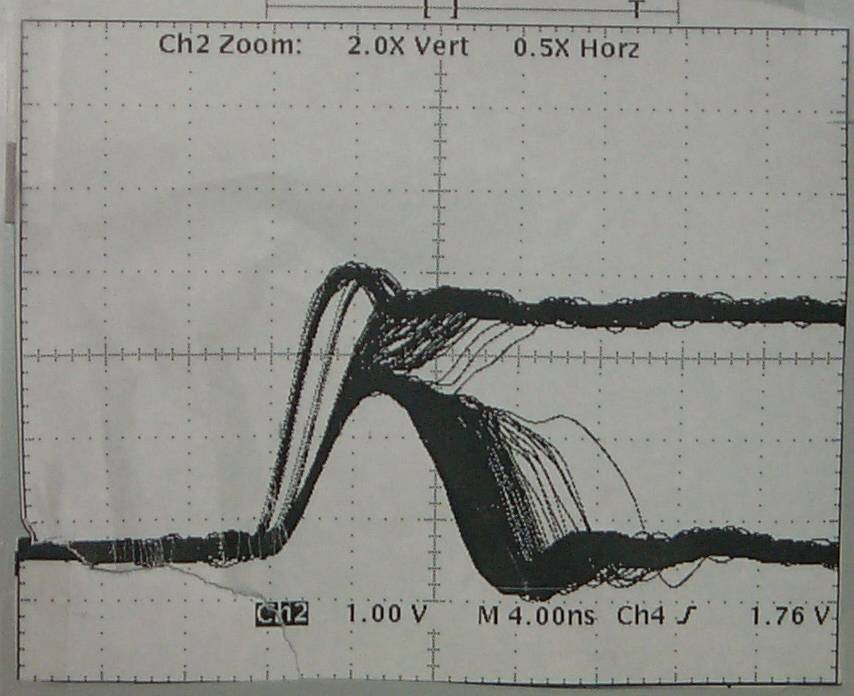
\includegraphics[scale=0.3]{figs/meta_pic.jpg} 
\caption{A practical example of metastability}
\label{fig:meta}
\end{figure}

Synchronization is generally done by passing the input value into one or more flip-flop's which is synchronized to the clock. Some signals in our design (\texttt{coin1}, \texttt{coin2}, \texttt{coin5} and \texttt{buy}) not only need to be synchronized with the clock, but also need their pass-on signal to be activated for exactly one clock cycle only. This is due to the fact that even though you press a button for only as short a while as you are able to, the clock still ticks at about 760Hz which, in almost every situation, will lead to an active input for several clock cycles. This 1-clockcycle-active is done by running the signal through 2 consecutive flip-flops and only letting the pass-on signal go high as long as the output of the first flip-flop is high and the output from the second flip-flop is low. In order to get the pass-on signal activated again, the input signal needs to be turned off first. 

\subsection{Implementing the display-driver}
To begin with as a part of the lab-exercises in this course we implemented the display-driver as a 'Hexadecimal to seven-segment display' state machine, having one state per possible hexadecimal. This was implemented as a Process in VHDL. When the 4-bit binary input \texttt{d} changes value (see Appendix A - display\_driver), the LED's of the display reflects the change.\\

\begin{figure}[!h]
\centering

\includegraphics[scale=0.5]{figs/single_digit_1.png} 
\caption{The representation of the 4-bit binary value "0001"}
\label{fig:single_digit_1}
\end{figure}

In order to display hex-numbers on a seven-segment display, we have build a combinational circuit in VHDL to convert a 4-bit binary number into the patterns which represent the number on a single seven-segment display. \\

There is no clever logic between the input and output in this case, since the LED's needed to display the different characters have no logical relation to the value that needs to be on the display. 
Therefore the implementation is a direct implementation of the state-table. \\

We implemented our state-table in a \texttt{Process(d)}. The input signal \texttt{d} is represented as an \texttt{UNSIGNED} 4-bit-vector. This process has a nested case statement, which represents the truth table. \\

The signal \texttt{led} is an \texttt{UNSIGNED} 8-bit-vector, 7-bits for the lines and one for the dot. \\

In this frame the first two lines of the \texttt{Process(d)} is show.
\begin{framed}
\texttt{
Case d IS \\
	WHEN "00000" => led <= NOT "11111100"; -- 0 \\
	WHEN "00001" => led <= NOT "01100000"; -- 1 \\
}
\end{framed}

\subsubsection{Expanding design to binary-coded-decimal instead of hexadecimal}
This hex-design was quickly abandoned, as it is not practical to read a price-tag in hexadecimal. Therefore we expanded our design to display binary-coded-decimal (BCD) values on the display instead. \\

The seven-segment logic was left untouched as the displays still must be able to display the numbers from 0-9, the hex-decimal-states was left untouched but is not used in our design. Later the state table was expanded further to enable us to display the characters needed for the displaying of product-names. See appendix A, figure \ref{vhd:dispdriv1}.

The input word \texttt{(d)} was changed from a 4-bit \texttt{UNSIGNED} to a 5-bit \texttt{UNSIGNED}. \texttt{d} had to be expanded to make room for the ekstra characters needed for the product names.

Further more the input values to display \texttt{price} 
This allows the two 2-decimal displays (price \& sum) to display values between 0-63.

\subsubsection{Time multiplexing the four seven-segment-displays}
To enable the displays to represent four different values to the user time multiplexing was implemented. Time multiplexing means cycling through the displays, turning them on one by one and displaying the corresponding value on the target display. \\

This is implemented by a 2-bit counter, incremented by the rising\_edge of the clock. The 2-bit overflow makes sure that the counter-value \texttt{m} stays between 0-3. The counter is incremented like so: \texttt{m\_next <= m + 1}. This counter is used a the selector to a multiplexer, selecting the right value for the corresponding display. The counter-value \texttt{m} also controls which display-anode \texttt{(an)} is turned on. Thus, each display is only turned on when it's value is represented on the 8-bit \texttt{led}-vector.

\subsection{Implementing the Processing Unit}

The Processing Unit is the central arithmetic core unit of the vending machine. This component calculates the total amount of coins inserted, and determines whether or not enough coins are inserted to purchase a product and if this is the case, subtracts the product of price from the total amount inserted. The Processing Unit is also the component taking care of asserting an alarm signal if a buy is attempted with too low total coin amount inserted as well as setting a the price and displaying the product name when a product is chosen. Below it is explained how the Processing Unit operates when one of the four different types of inputs are asserted:

\begin{itemize}
\item If \texttt{Reset} is asserted the sum will be set to zero.
\item If one of the three \texttt{price\_product} signal are asserted the \texttt{product} signal will be set to 1 for limited time period. This will cause the \texttt{price\_out} signal to be set to the value of the product as well as displaying the name of the product on the LEDs for as long as \texttt{product} is 1.
\item If one of the three \texttt{coin} input signal are asserted the Processing Unit will cause the sum signal to be incremented by the value of the coin inserted.
\item If the \texttt{buy} input is asserted, the machine will calculate whether buy is greater than or equal to price. If this is the case a \texttt{release\_can} signal is set to 1 and the price is subtracted from the sum. Notice that the \texttt{sum} signal won't be set to zero after a successful buy, because the machine is designed in such a way that it doesn't give back money (a good business design!). On the other hand if the \texttt{buy} input is asserted when sum is less than price, the alarm signal will be set to 1 for a limited amount of time, causing the display to blink on a 3 Hz clock for a approximately a couple of seconds. Notice here that the alarm counter \texttt{alarm\_count} runs on the normal 763 Hz clock and therefore the alarm signal is not synchronized to the 3 Hz clock, meaning that the alarm signal can start and stop in the middle of a 3 Hz clock period.
\end{itemize}

In the \texttt{process(coin1, coin2, coin5, buy, clock)}, we have chosen nested if else statements so that Reset have highest precedence, then the coins, then alarm and finally buy. It's obvious that we want Reset to overrule all other inputs, but the coin inputs have higher precedence than alarm as you would always want a machine to register when coins are inserted even though the alarm is on (unless you a mean business man!). buy however has lower precedence than alarm, as we want the machine to stop alarming (aka blinking) before another buy can be attempted. \\

To test whether the written VHDL code for this component works as intended, we simulate it in the ModelSim environment. This is done by writing a .do file for ModelSim, which sets the input signals to relevant combinations, and simulating clock signals. By doing this it is tested if the output signals are as intended. The .do file can be seen in figure \ref{fig:dofile}.

\begin{figure}[h!]
\centering
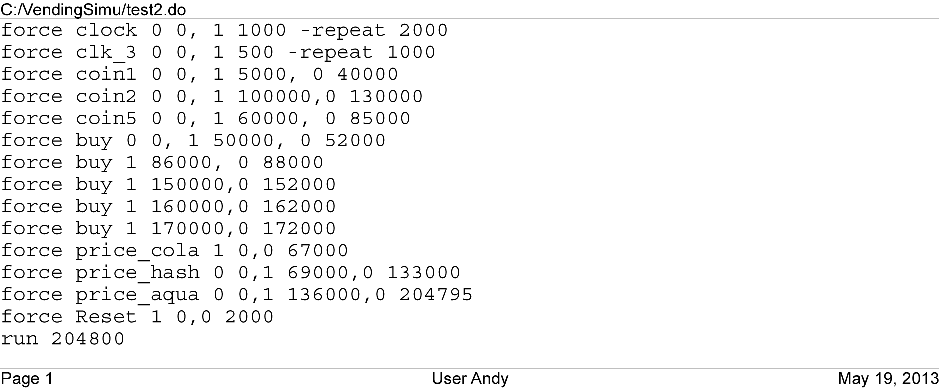
\includegraphics[scale=0.8]{figs/dofile.pdf}
\caption{Do-file for the Processing Unit ModelSim simulation}
\label{fig:dofile}
\end{figure}

The timing diagram in figure \ref{fig:simu}. is imported from ModelSim and shows the simulated components response to different inputs. As expected the \texttt{price\_out} changes to the wanted value when a product signal is switched on. It is also seen that \texttt{cola\_out}, \texttt{hash\_out} and \texttt{aqua\_out} respectively is set to 1 when the when the price switch for each of the products is asserted. This is the signal which are passed on to the display driver, which writes the product name on the display. Since the name is set to be there for approximately 2 seconds, this simulation does not show that these -\texttt{\_out} signal are de-asserted after this period of time, since the simulation only cover 0.002 s, even though the simulation clock ticks faster. It is also seen that the calculating mechanism works correctly since the price is subtracted from the sum and yields the correct value, when buy is asserted. It is seen as well that the \texttt{alarm\_out} signal is asserted (in the last case where price is higher than sum) exactly as it should. It should be remembered that these signals have not been through the input synchronizer which ensure that coin, buy and price signals only are set to one for a single clock period when activated on the Basys board.

\begin{figure}[h!]
\centering
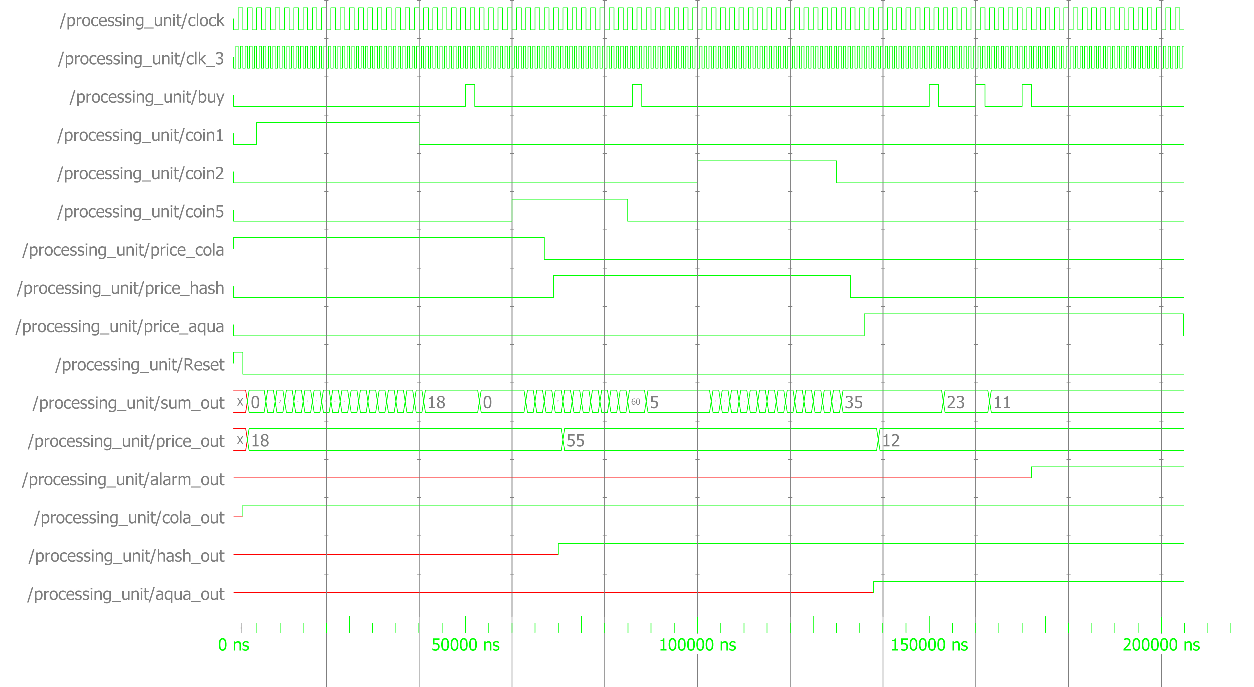
\includegraphics[scale=0.8]{figs/processingunit.pdf}
\caption{Timing Diagram for the ModelSim simulation}
\label{fig:simu}
\end{figure}

\subsection{The structure of the Vending Machine}

The overall structure of the vending machine can be seen in vending\_machine.vhd-file. Here the signals of the different components are tied together to the overall basys-board input and output signals. The components included in vending\_machine.vhd includes the clock\_manager.vhd, display\_driver.vhd, input\_synchronizer.vhd and processing\_unit.vhd \\

Generally the overall structure is that the input signals from the Basys board are connected to the input\_synchronizer to make the signal go high for only one clock cycle when one of the switches or buttons are asserted. Next the signals are sent to the processing unit to compute sum, price, alarm and so on and then finally to display\_driver where the signals are connected back to the Basys board.\\

\begin{figure}[h!]
\centering
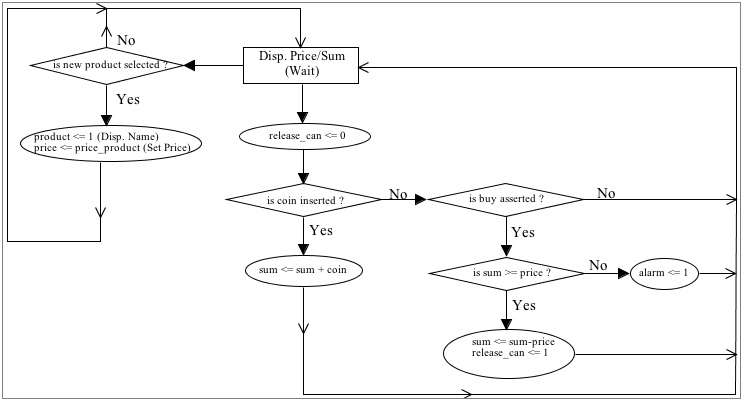
\includegraphics[scale=0.6]{figs/asm_chart.png}
\caption{ASM-Chart showing the overall functionality of the vending machine}
\label{fig:asm}
\end{figure}

On figure \ref{fig:asm} the overall functionality of the Vending Machine is displayed as an ASM-Chart. The machine has 'wait' state where price and sum is displayed. The machine will remain in this state until either a coin is inserted, a product is selected or a buy is attempted. If a product is selected, the product name will be displayed and a the price of that specific product will be set. If a coin is inserted sum will be incremented by the coins value. If buy is asserted and sum is less than price, the alarm signal will be set to 1 causing the both price and sum on the display to blink for a while. If sum is greater than or equal to price, the release\_can signal is set to 1 and sum is subtracted the value of that specific product.